\section{Auswertung}
\label{sec:Auswertung}

\begin{figure}
  %Plot der Messwerte aus a)
  \centering
  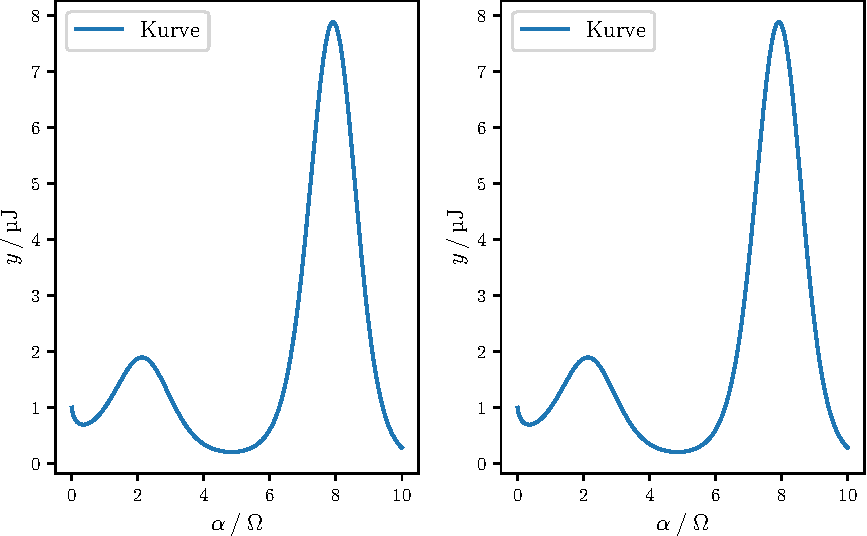
\includegraphics{plot.pdf}
  \caption{Plot.}
  \label{fig:plot}
\end{figure}

\begin{table}
  %Messwerte aus a)
  \centering
  \caption{Tabelle der Messwerte mit \(R_1\).}
  \label{tab:tab1}
  \begin{tabular}{c c}
    \toprule
    U in $V$ & t in $\mu$s\\
    \midrule
    0.2 & 0\\
    0.14 & 25\\
    0.1 & 54\\
    0.07 & 78\\
    0.05 & 105\\
    0.04 & 130\\
    0.03 & 158\\
    0.02 & 184\\
    0.014 & 210\\
    0.008 & 247\\
    \bottomrule
  \end{tabular}
\end{table}

\begin{table}
  %Messwerte aus c)
  \centering
  \caption{Tabelle der Messwerte mit \(R_2\)}
  \label{tab:tab2}
  \begin{tabular}{c c}
    \toprule
    $\nu$ in $kHz$ & U in $V$\\
    \midrule
    5 & 0.8\\
    10 & 0.85\\
    15 & 0.9\\
    20 & 1\\
    25 & 1.2\\
    30 & 1.6\\
    35 & 2\\
    40 & 1.7\\
    45 & 1.1\\
    50 & 0.75\\
    55 & 0.55\\
    60 & 0.43\\
    65 & 0.34\\
    70 & 0.28\\
    75 & 0.24\\
    \bottomrule
  \end{tabular}
\end{table}

\begin{figure}
  %Plot der Messwerte aus c)
  \centering
  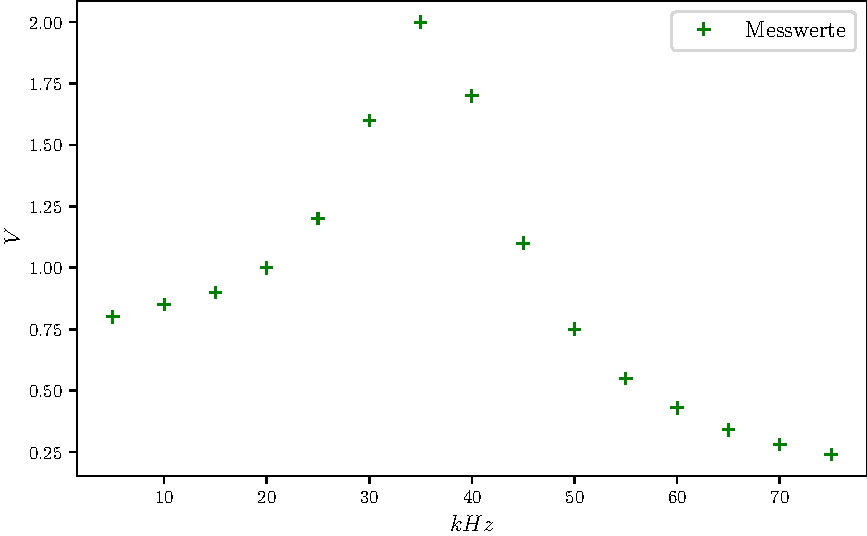
\includegraphics{plot2.pdf}
  \caption{Plot2.}
  \label{fig:plot2}
\end{figure}

\begin{table}
  %Messwerte aus d)
  \centering
  \caption{Tabelle der Messwerte mit Phasenunterschied.}
  \label{tab:tab3}
  \begin{tabular}{c c c}
    \toprule
    $\nu$ in $kHz$ & a in $\mu$s & b in $\mu$s\\
    \midrule
    140 & 0.08 & 7\\
    120 & 0.1 & 8\\
    100 & 0.2 & 10\\
    80 & 0.3 & 11\\
    60 & 0.8 & 15.5\\
    40 & 4.2 & 22.5\\
    \bottomrule
  \end{tabular}
\end{table}

\begin{table}
  %Messwerte aus c) mit Delta Phi
  \centering
  \caption{Tabelle der Messwerte mit \(\Delta\phi\)}
  \label{tab:tab4}
  \begin{tabular}{c c}
    \toprule
    $\nu$ in $kHz$ & $\Delta\phi$ in °\\
    \midrule
    140 & 67.2\\
    120 & 18.58\\
    100 & 9.82\\
    80 & 7.2\\
    60 & 4.5\\
    40 & 4.11\\
    \bottomrule
  \end{tabular}
\end{table}

\begin{figure}
  %Plot zu Messwerten aus d)
  \centering
  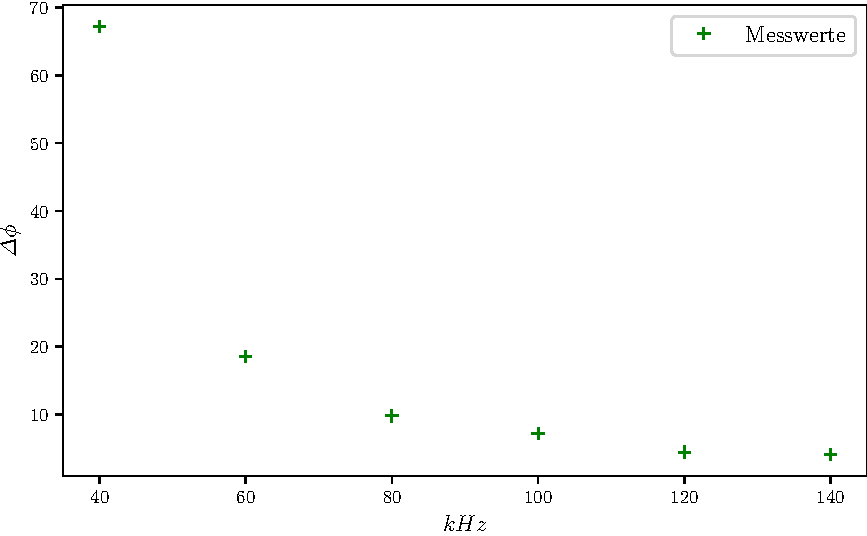
\includegraphics{plot3.pdf}
  \caption{Plot3.}
  \label{fig:plot3}
\end{figure}

Siehe \autoref{fig:plot}!
